% !TEX program = xelatex
% [EN] The notes and slides share the same physics and source definitions. / [CN] 讲稿与幻灯片共用物理内容和来源定义。
\ifdefined\SpeakerNotes
  \documentclass[12pt,a4paper]{article}
  \usepackage[margin=24mm]{geometry}
  \usepackage{hyperref}
\else
\documentclass[aspectratio=169,14pt]{beamer}
  \geometry{paperwidth=320mm,paperheight=180mm}
\fi
\usepackage{lmodern,fontspec,xeCJK}
\setmainfont{TeX Gyre Heros}
\setsansfont{TeX Gyre Heros}
\setCJKmainfont{Noto Sans CJK SC}
\setCJKsansfont{Noto Sans CJK SC}
\usepackage{amsmath,amssymb,booktabs,tabularx,array,graphicx,xcolor}
\definecolor{Navy}{HTML}{16324D}
\definecolor{Teal}{HTML}{007F86}
\definecolor{Ink}{HTML}{26323B}
\definecolor{Muted}{HTML}{586974}
\definecolor{Rust}{HTML}{A14D22}
\hypersetup{colorlinks=true,urlcolor=Teal,linkcolor=Teal,
 pdftitle={Polarized deuteron beam preparation for SAMURAI},pdfauthor={Baiting Tian}}
\newcolumntype{Y}{>{\raggedright\arraybackslash}X}
\newcommand{\src}[2]{\href{#1}{#2}}
\newcommand{\sakamoto}{https://proceedings.jacow.org/cyclotrons2016/papers/tub04.pdf}
\newcommand{\okamura}{https://www.nishina.riken.jp/researcher/APR/Document/ProgressReport_vol_28.pdf}
\newcommand{\sugahara}{https://indico.cern.ch/event/1441702/contributions/7106564/}
\newcommand{\avftest}{https://indico.ibs.re.kr/event/701/contributions/6590/}
\newcommand{\fthreelimit}{https://www.nishina.riken.jp/ribf/BigRIPS/intensity.html}
\newcommand{\bis}{https://www.nishina.riken.jp/researcher/APR/APR058/pdf/98.pdf}
\newcommand{\attlocations}{https://www.nishina.riken.jp/researcher/APR/APR047/pdf/156.pdf}
\newcommand{\slitsource}{https://www.nishina.riken.jp/researcher/APR/APR052/pdf/130.pdf}
\newcommand{\attguide}{https://ribf.riken.jp/sisetu-kyoyo/HIbeam/BmL/BmL\%E4\%BD\%9C\%E6\%96\%B9111__\%E7\%90\%86\%E7\%A0\%94\%E3\%81\%AE\%E5\%A0\%B4\%E5\%90\%88.pdf}
% [EN] Ideal RF modes must remain distinct from measured polarization and current operating setpoints. / [CN] 理想 RF 模式须与实测极化及当前控制设定明确区分。
\newcommand{\noteone}{%
先区分氘原子和氘核。PIS 解离 $\mathrm D_2$ 后形成的是中性氘原子束，此时每个原子还有一个电子。基态电子的轨道角动量 $L=0$，所以 $J=S=1/2$，有两个自旋投影；氘核 $I=1$，有三个投影。因此联合自旋空间的维数为 $(2S+1)(2I+1)=2\times3=6$。

零场时，电子与核自旋通过超精细作用耦合，总角动量 $\mathbf F=\mathbf I+\mathbf S$。$F=3/2$ 有四个 $m_F$ 子态，$F=1/2$ 有两个。这是六个子态、两个零场能量，并非零场就有六个不同能量。

沿局部静磁场方向取量子化轴，哈密顿量可写为
\[
 H_0=\frac{A}{\hbar^2}\,\mathbf I\!\cdot\!\mathbf S
     -(\boldsymbol\mu_e+\boldsymbol\mu_d)\!\cdot\!\mathbf B_0.
\]
第一项是超精细耦合，第二项是 Zeeman 相互作用。改变 $B_0$ 会改变六条能量分支 $E_i(B_0)$ 及本征态的混合，这就是右侧 Breit--Rabi 图。

在强场极限，可以用 $|m_S,m_I\rangle$ 理解各态：1、2、3 的 $m_S=+1/2$，$m_I$ 依次为 $+1,0,-1$；4、5、6 的 $m_S=-1/2$，$m_I$ 依次为 $-1,0,+1$。因此状态 3 和 6 分别趋向核自旋投影 $-1$ 和 $+1$。图中的 $m_j$ 与这里的 $m_S$ 等价。

弱场下应使用耦合态。常用编号中，1--4 属于 $F=3/2$，$m_F$ 依次为 $+3/2,+1/2,-1/2,-3/2$；5、6 属于 $F=1/2$，$m_F$ 分别为 $-1/2,+1/2$。除伸展态等特殊情况，一般不能把弱场态当成一个确定的 $m_S,m_I$ 组合。编号 1--6 是连续跟踪的原子态标签。

这一页要建立的联系是：静磁场决定能级间距，RF 单元利用这些间距重新分配原子态布居；下一页再解释这些布居怎样变成氘核极化。

\textbf{来源：}\src{\hyperfineref}{Sabourov, Duke PhD thesis (2006), Sec. 2.1.2, pp. 22--23, Fig. 2.3 / PDF pp. 46--47}；\src{\rfprinciple}{Mikirtychyants et al., arXiv:1212.1840, Sec. II G, pp. 7--8}。
}

\newcommand{\notetwo}{%
RF 是控制布居的旋钮。对允许的单光子磁偶极跃迁，$h\nu=|E_j(B_0)-E_i(B_0)|$ 给出共振条件。绝对值同时涵盖吸收和受激发射。还必须有非零耦合 $\langle j|\boldsymbol\mu\cdot\mathbf B_1|i\rangle$；满足能量条件本身并不保证任意两态都能跃迁。RF 幅度、方向、原子通过时间和静场梯度共同影响转移效率，实际源常采用绝热通过共振的方式。

WFT 是 Weak Field Transition，在弱静场下耦合 $F$ 多重态中的相邻 $m_F$ 态。SFT 是 Strong Field Transition，用于不同超精细多重态相连分支间的跃迁。名称不是 RF 功率大小的分类；SFT 也不能简单理解成所有实际装置都工作在无限强场极限。具体工作点由能级间距和装置配方决定。

现在只看理想 $p_{yy}=+1$。第一组六极磁铁选择聚焦的电子自旋组，保留 1、2、3，排斥 4、5、6。理想等布居下，三个核投影仍各占一份。RF 和选择磁铁的配合才能得到所需布居；对六态完全等布居的体系，单纯的相干 RF 重排不会产生净极化。

接着 WFT\#1 实现有效的 $1\to4$ 布居转移。它通过中间态进行，不能把 $1\to4$ 当成直接的单光子跃迁：弱场的相邻步满足 $\Delta m_F=\pm1$。相应的 $2\leftrightarrow3$ 交换对这里相等的两份布居没有影响。WFT 后可用集合 $2,3,4$ 表示，第二组六极磁铁排斥 4，留下等布居的 2、3。

SFT\#2 再做 $2\to6$，进入 ECR 的状态变成等量的 3、6。ECR 去掉电子成为 $\mathrm D^+$。在理想强场与极化保持条件下，核布居是
\[
(n_+,n_0,n_-)=(1/2,0,1/2),\qquad
p_y=n_+-n_-=0,\quad p_{yy}=1-3n_0=+1.
\]
SFT\#1 和 WFT\#2 关闭。实际输出受选态、RF 转移和电离效率等影响，需测量 $p_y,p_{yy}$。RF 控制布居，Wien filter 控制轴向；我们保持源的竖直轴，不要求额外转轴，并确认输运到实验靶后的方向。对轴对称态仍有 $p_{xx}=p_{zz}=-p_{yy}/2$。

\textbf{来源：}\src{\rfprinciple}{Mikirtychyants et al., Sec. II G}；\src{\okamura}{Okamura et al., RIKEN APR 28 (1995), Table 1, p. 148 / PDF p. 179}；\src{\sakamoto}{Sakamoto et al., Cyclotrons 2016, pp. 145--146}。
}

% [EN] Defer the negative-tensor state explanation. / [CN] 暂不展示负张量态的说明。
% 负 tensor 理想态全部占据 $m_y=0$，给出 $p_{yy}=-2$，vector polarization 为零。
% [EN] Defer the negative-tensor transition and final states. / [CN] 暂不展示负张量模式的跃迁和最终态。
% 负 tensor 使用 SFT\#2 的 $3\to5$，最终为 2、5 态。
% [EN] Defer positive/negative tensor switching. / [CN] 暂不讨论正负张量模式切换。
% 原表脚注明确说，在 RF 频率固定时改变 SFT\#2 磁场，可以切换 $2\to6$ 和 $3\to5$。
% [EN] Defer the historical negative-mode measurement. / [CN] 暂不展示负模式的历史测量值。
% 负 tensor 模式的实测 tensor 分量约为 $-1.23$。

\newcommand{\notethree}{%
PIS 已有近期恢复运行的证据。2024 年 9 月在 AVF 后进行了 7 MeV/u 的极化测试。2026 年会议报告进一步说明，1 月已经在 100 MeV/u 完成极化束实验，报告 $p_y=-0.615\pm0.005$ 和 $p_{yy}=+0.896\pm0.012$。这个结果表明源和测偏系统有近期运行经验，但该模式含有 vector polarization。

我们要确认的是：假如无法获得 Sekiguchi 老师的帮助，RIKEN 是否有人员具备独立准备、调试和运行极化氘束的能力？这里的前提包括无法获得她的远程指导，不能假定她会预先完成关键调试。

需要具体确认的能力包括：启动和调节 PIS、设置纯 tensor RF 模式、调节加速与束流输运，以及测量和验证极化。常规氘束的调束经验能否覆盖我们要求的纯 tensor 极化氘束，是这次会议需要回答的问题。这些工作可以由 RIKEN 内不同人员共同承担。

N. Sakamoto 等 RIKEN 人员参与了公开报告，可以作为联系线索。近期实验说明系统有运行经验，但仅凭署名无法确认 RIKEN 团队能否在没有 Sekiguchi 老师帮助的情况下独立完成这些工作。希望会议明确回答是否具备这一能力，由谁负责，以及需要多少准备时间和调束时间。

\textbf{建议口头问题：}Can RIKEN staff independently prepare and tune the polarized deuteron beam, including this pure-tensor RF mode and polarization checks, without assistance from Prof. Sekiguchi?

\textbf{来源：}\src{https://www.nishina.riken.jp/researcher/APR/APR058/pdf/36.pdf}{Sugahara et al., RIKEN APR 58 (2025), p. 36}；\src{\sugahara}{Sugahara et al., EFB 2026, January 2026 run and authors}。
}

\newcommand{\notefour}{%
这里比较的是三个可供选择或互相补充的位置。应先确认现有设备能否使用，再决定新装探测器的工作量。

AVF 后的 polarimeter 适合检查源的模式和极化。2024 年测试通过 $^{12}\mathrm C(d,p)^{13}\mathrm C$ 反应测偏，束流随后停在 Faraday cup。因此需要确认它是否支持向 RRC 连续送束时的测量，还是需要独立的测偏时段。还要检查本次 AVF 引出能量对应的标定。

RRC 后、SRC 前在历史束流布局中已有 DPOL，这是建议优先询问的现有装置。需确认位置是否位于本次实际输运路径、硬件和 DAQ 是否可用，以及标定能量和测偏靶对 SRC 注入的影响。2026 年实验的 D-room polarimeter 不能未经位置核实就等同于这台输运线 DPOL。

SRC 后可以直接测最终加速能量下的束流极化，也更接近我们计划安装探测器的方案。要确认具体空间、真空接口，以及该处允许的束流强度。

任何上游测偏都需要与 SAMURAI 实验靶处建立联系。后续磁场输运和相空间选择可能改变轴向或透过束的平均极化。本页不把上游结果直接当成最终靶处的实测值。

\textbf{建议口头问题：}Can we use an existing polarimeter after AVF or RRC, and can it operate with the beam delivery required for our experiment?

\textbf{来源：}\src{\sakamoto}{Sakamoto et al., 2016, Fig. 1, historical DPOL and BigDPOL layout}；\src{\avftest}{Sugahara et al., INPC 2025, AVF measurement setup}。
}

\newcommand{\notefive}{%
BigRIPS 的官方说明给出 F3 总束流率不超过 $10^7$/s。我们的理想布置是在 SRC 后保留较高强度用于测偏，然后在 F3 之前衰减。这样是否允许，要同时看实际束流和联锁条件。

ATT 是网格束流衰减器。穿过网孔的粒子避免直接穿过板材，部分束流则被网格截获。RIKEN 列出 $1/2$、$1/3$、$1/5$、$1/10$ 和 $1/100$ 等名义透过率。它们不能自动代表实际端到端透过率，尤其不能直接外推到高能氘束。文献中的 C22、S31a、S64 位于 RRC 上游，在这些位置衰减也会降低 SRC 后的测偏计数率。

狭缝可以减小接受度。F2--F3 的狭缝选择角度，色散位置的狭缝还可能选择动量。所需开口必须结合束流分布计算。举例：居中一维高斯束、$\sigma=1$ mm，透过率 $T=\operatorname{erf}[w/(2\sqrt2\sigma)]$，$T=0.01$ 对应全开口 $w\simeq25\,\mu$m。若两个独立方向各透过 10\%，每个全开口约 0.25 mm。这只是理想算例。

更关键的是，2025 年 BIS 报告描述了利用上游 ATT 插入状态判断是否允许一次束进入 BigRIPS 的逻辑，衰减不足时会插入 SRC 出口 Faraday cup。所以狭缝将 F3 实测速率降下来，未必满足现有送束条件。必须确认当前配置能否接受我们提出的位置和衰减方案，以及截获束流、散射背景和透过束极化的影响。

\textbf{建议口头问题：}Can we retain a higher rate at the after-SRC polarimeter and attenuate before F3 under the applicable interlock configuration?

\textbf{来源：}\src{\fthreelimit}{F3 official limit}；\src{\attguide}{RIKEN intensity guide, p. 7}；\src{\attlocations}{APR 47, p. 156}；\src{\slitsource}{APR 52, p. 130}；\src{\bis}{APR 58, pp. 98--99}。
}

\newcommand{\noteprecisionreference}{%
这一页把原来的 10 s 和 60 s 两张图并排比较，作为后面提高测偏束流强度的基准。横轴为真实 $p_{yy}$，纵轴为期望计数构成的典型数据所给出的参数置信区间。深色、浅色分别为名义 68.3\% 和 95\% 区间。色带不是重复测量估计值的分布。

沿用当前配置：190 MeV/u，$I_{\rm pol}\simeq10^7$ d/s，CH$_2$ 面密度暂取 1000 mg/cm$^2$。使用 $53.4^\circ$/205 mm 的质子臂与 $20.9^\circ$/140 mm 的氘核臂的符合计数。20 mm 探测器仍采用已有的 $20\times20$ mm 接受度近似。

对每个真实值 $p_0$，令 $N_{LR}=\mu_{LR}(p_0)$、$N_{UD}=\mu_{UD}(p_0)$，不对非整数期望计数取整。使用条件二项似然
\[
q(p)=\frac{\mu_{LR}(p)}{\mu_{LR}(p)+\mu_{UD}(p)},\qquad
\ell(p)=N_{LR}\ln q(p)+N_{UD}\ln[1-q(p)].
\]
两种区间对应 $-2\Delta\ell\leq1$ 和 $3.84146$。这是现有 C++ 推断方法的一参数渐近阈值，图中的 68.3\% 是 68.27\% 的四舍五入。

当真实 $p_{yy}=1$，基准计数与区间为：
\precisiontable{}

60 s 的期望计数是 10 s 的六倍，远离边界的统计误差约为其 $1/\sqrt6$。拟合保留物理域 $[-2,1]$，仅显示真实值 $[0,1]$；区间可以延伸到负值，或在上端达到 1。边界处的名义置信度不代表已经校准的精确覆盖率。

所有图只包含计数统计，固定分析本领和相对扇区响应，假定单位效率与活时间，没有背景或能损修正。后两页仅把 LR、UD 两类期望计数同时乘以 10 或 100，不改变这些假设。

{\small\textbf{计算来源：}\par
配置：\path{code/config/current_tensor.ini}\par
前向模型与推断：\path{code/src/counts.cpp}；\path{code/src/inference.cpp}\par
作图和摘要：本目录 \path{plot_pyy_confidence.py}\par}
}

\newcommand{\noteprecisiongainTen}{%
这一页假设 ATT 或 slits 放在 polarimeter 下游、F3 上游，透过率为 1/10。在 F3 仍维持约 $10^7$ d/s 的情况下，polarimeter 处可以使用约 $10^8$ d/s。于是同样时间内测偏计数为基准的十倍。

计算仅作归一化变化：
\[
\mu_{LR}^{(10)}(p)=10\mu_{LR}^{(1)}(p),\qquad
\mu_{UD}^{(10)}(p)=10\mu_{UD}^{(1)}(p).
\]
束流时间仍为 10 s 和 60 s。计数比的中心值不变，而似然曲线变窄。以放大后的期望计数重新计算同样的 68.3\%、95\% 区间，没有将区间宽度直接乘以某个倍率。

当真实 $p_{yy}=1$：
\precisiontable{GainTen}

左图和右图分别与上一页的 10 s、60 s 对照。固定时间、远离边界时，统计误差约为基准的 $1/\sqrt{10}\simeq0.316$。这反映增加有效统计量的收益。

该假设要求衰减发生在测偏之后。如果 ATT 在源或加速器上游先把束流削弱，就不会获得这里的测偏计数增益。束线和联锁能否采用这一位置安排仍需确认。图中仍按参考方案的几何、效率、活时间和背景假设计算。

\textbf{计算来源：}同基准页。生成摘要记录计数倍率 10，逐点核对 LR、UD 计数确为基准的十倍。PDF 与 TeX 同级保存。
}

\newcommand{\noteprecisiongainHundred}{%
这一页把下游 ATT / slits 的透过率假设改为 1/100。为使 F3 维持约 $10^7$ d/s，polarimeter 处束流取约 $10^9$ d/s，对应基准计数的百倍。左右两图仍分别为 10 s 和 60 s。

计算只把两类计数共同放大：
\[
\mu_{LR}^{(100)}(p)=100\mu_{LR}^{(1)}(p),\qquad
\mu_{UD}^{(100)}(p)=100\mu_{UD}^{(1)}(p).
\]
真实 $p_{yy}$ 扫描范围、几何和分析本领完全相同。单纯提高归一化不改变期望计数比，也不改变 Asimov 最佳拟合值。

当真实 $p_{yy}=1$：
\precisiontable{GainHundred}

固定时间、远离边界时，统计误差大致缩小到基准的 $1/10$。六张图使用相同坐标范围，所以百倍统计的色带会显得很窄，表格列出了端点供精确比较。

这是保持原有效效率和活时间的条件估计。衰减器位置、可用的上游强度及束线联锁需满足前述方案；本页不额外模拟 ATT 或狭缝造成的接受度、背景或极化变化。实际增益应以有效计数是否按比例增长为准。

\textbf{计算来源：}同基准页。生成摘要记录计数倍率 100，并检查置信区间端点和相对基准的计数缩放。
}

\newcommand{\notesix}{%
希望这次会议确定的事项有四类。第一是如果无法获得 Sekiguchi 老师的帮助，RIKEN 是否有人员能独立完成极化氘束调试，由谁负责，以及需要多少准备时间。第二是可用的纯 tensor RF 配方、允许的残余 $p_y$，以及保持竖直轴的输运设置。第三是测偏设备的位置、可借用的硬件和测量周期。第四是允许的束流强度、衰减位置和对应联锁条件。

“需要高计数率”还要转换成一个可以评估的要求。薄靶近似下，有效计数率可写成
\[
R_{\rm useful}=\dot N_{\rm pol}\,n_t\,\sigma_{\rm acc}\,\epsilon\,f_{\rm live}.
\]
这里 $\dot N_{\rm pol}$ 是测偏靶处粒子率，$n_t$ 是相关散射中心的面密度，$\sigma_{\rm acc}$ 是接受范围内的有效截面，$\epsilon$ 是未重复计入接受度的探测和选择效率，$f_{\rm live}$ 是活时间比例。若这些因素不能近似分离，需要做联合的接受度积分。CH$_2$ 靶还需要考虑碳背景。

高束流可以缩短同样计数所需的时间，但极化误差还取决于分析本领、角度覆盖、背景和归一化。前三页曲线比较了基准、十倍和百倍计数下，10 s 与 60 s 的典型数据置信区间；这些是附带假设的设计估计。还需确认实际束流强度、靶厚、效率与所需 $p_{yy}$ 精度，才能确定正式监测周期。

如果现有联锁要求在上游就把束流降到很低，应进一步讨论接受度和靶厚是否足以满足周期要求，或能否安排独立的测偏时段。测偏时段与正式送束的设置差异及极化稳定性需要交叉检查。

\textbf{建议结束语：}With the source support, polarimeter location, and permitted intensity agreed, we can calculate the measurement time needed for the requested polarization precision.

\textbf{来源：}本页为本次会议的决策请求。计数率表达式为薄靶近似下的标准通量--截面关系。此前的曲线采用当前配置中的暂定参数。
}


\ifdefined\SpeakerNotes
  \setlength{\parindent}{0pt}
  \setlength{\parskip}{0.7em}
  \setlength{\emergencystretch}{2em}
  \newcommand{\notepage}[3]{
    {\color{Muted}\small SAMURAI meeting \quad 中文讲稿 \quad #1/6\par}
    \vspace{0.6em}{\color{Navy}\LARGE\bfseries #2\par}\vspace{0.7em}
    #3
  }
\else
\setbeamercolor{normal text}{fg=Ink,bg=white}
\usefonttheme{professionalfonts}
\setbeamercolor{frametitle}{fg=Navy,bg=white}
\setbeamercolor{structure}{fg=Teal}
\setbeamercolor{alerted text}{fg=Rust}
\setbeamerfont{normal text}{size=\fontsize{20}{25}\selectfont}
\setbeamerfont{frametitle}{size=\fontsize{32}{37}\selectfont,series=\bfseries}
\setbeamersize{text margin left=13mm,text margin right=13mm}
\setbeamertemplate{navigation symbols}{}
\setbeamertemplate{frametitle}{\vspace{5mm}\insertframetitle\par\vspace{3mm}}
\setbeamertemplate{footline}{\hspace{13mm}{\color{Muted}\fontsize{10}{12}\selectfont SAMURAI beam preparation\hfill\insertframenumber/6\hspace{13mm}}\vspace{4mm}}
\newcommand{\smalltext}{\fontsize{17}{22}\selectfont}
\newcommand{\source}[1]{\vfill{\color{Muted}\fontsize{10}{13}\selectfont #1\par}}
\newcommand{\lead}[1]{{\color{Teal}\bfseries #1\par}\vspace{3mm}}
\renewcommand{\arraystretch}{1.35}
\title{Polarized deuteron beam preparation for SAMURAI}
\author{Baiting Tian}
\date{10 September 2026}
\fi
\begin{document}
\ifdefined\SpeakerNotes
    \notepage{1}{我们需要怎样的极化氘束}{\noteone}\clearpage
    \notepage{2}{纯 tensor 模式的 RF 跃迁}{\notetwo}\clearpage
    \notepage{3}{RIKEN 能否独立完成极化氘束调试}{\notethree}\clearpage
    \notepage{4}{三个测偏位置的比较}{\notefour}\clearpage
    \notepage{5}{F3 限制、ATT 与狭缝}{\notefive}\clearpage
    \notepage{6}{希望这次会议确定的事项}{\notesix}
\else
\usebeamerfont{normal text}

\begin{frame}[t]{Vertical pure-tensor deuterons for SAMURAI}
\lead{Requested mode: ideal $(p_y,p_{yy})=(0,+1)$, with the symmetry axis along vertical $y$}
\begin{columns}[T,onlytextwidth]
\column{0.53\textwidth}
\vspace{1mm}
\[
 p_y=n_+-n_-,\qquad p_{yy}=n_++n_--2n_0
\]
\vspace{2mm}
\begin{tabularx}{\linewidth}{@{}Yccc@{}}
\toprule
Ideal mode & $n_+$ & $n_0$ & $n_-$\\
\midrule
$p_{yy}=+1$ & $1/2$ & $0$ & $1/2$\\
% [EN] Defer the negative-tensor population row. / [CN] 暂不展示负张量模式的布居。
% $p_{yy}=-2$ & $0$ & $1$ & $0$\\
\bottomrule
\end{tabularx}\par
\vspace{5mm}
\smalltext
For an axially symmetric state,\par
\vspace{1mm}
$p_{xx}=p_{zz}=-p_{yy}/2$.\par
\vspace{3mm}
An unpolarized reference has $n_+=n_0=n_-=1/3$.
\column{0.43\textwidth}
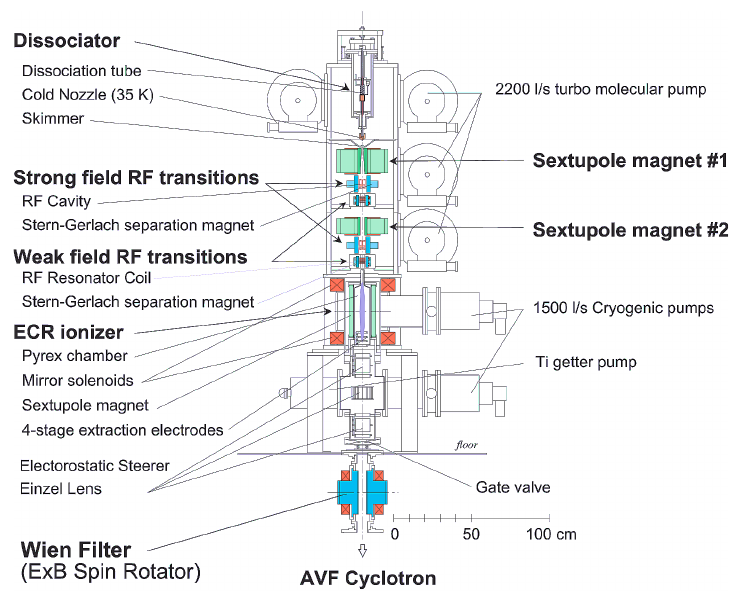
\includegraphics[width=\linewidth,height=58mm,keepaspectratio]{../../physics/polarization_production_transport/figures/sakamoto2016_p1_fig2.png}\par
\vspace{3mm}
\smalltext
The PIS ionizer output has a vertical polarization axis.\par
\vspace{3mm}
\textbf{No additional Wien-filter rotation requested.}\par
\vspace{2mm}
Confirm vertical-axis transport to the experimental target.
\end{columns}
\source{Source and original PIS drawing: \src{\sakamoto}{Sakamoto et al., Cyclotrons 2016, pp. 145--146, Fig. 2}. Ideal spin-1 populations are definitions, not measured source performance.}
\note{\noteone}
\end{frame}

\begin{frame}[t]{RF transitions for pure tensor polarization}
\lead{Historical RIKEN recipe for the ideal $(p_y,p_{yy})=(0,+1)$ mode}
\smalltext
SFT = strong-field transition. WFT = weak-field transition.\par
\vspace{4mm}
\begin{tabularx}{\textwidth}{@{}p{60mm}*{4}{>{\centering\arraybackslash}X}@{}}
\toprule
Ideal $(p_y,p_{yy})$ & SFT\#1 & WFT\#1 & SFT\#2 & WFT\#2\\
\midrule
$(0,+1)$ & Off & $1\to4$ & $2\to6$ & Off\\
% [EN] Defer the negative-tensor RF recipe. / [CN] 暂不展示负张量模式的 RF 配方。
% $(0,-2)$ & Off & $1\to4$ & $3\to5$ & Off\\
\bottomrule
\end{tabularx}\par
\vspace{6mm}
\begin{columns}[T,onlytextwidth]
\column{0.49\textwidth}
\textbf{State selection}\par
\vspace{2mm}
After the second sextupole: states $2,3$.\par
\vspace{2mm}
Final states: $3,6$ for $p_{yy}=+1$.
% [EN] Deferred negative-mode final states. / [CN] 暂不展示负模式的最终态。
% Final states: $2,5$ for $p_{yy}=-2$.
\column{0.47\textwidth}
\textbf{Current setup to confirm}\par
\vspace{2mm}
RF frequency, SFT\#2 magnetic field, and transition efficiency.
% [EN] Defer switching between positive and negative tensor modes. / [CN] 暂不讨论正负张量模式之间的切换。
% Keep the RF frequency fixed and change the SFT\#2 magnetic field.
\end{columns}
\vspace{6mm}
{\color{Teal}\bfseries Meeting request}\par
\vspace{2mm}
Confirm the current RF recipe and achievable $p_{yy}$, including residual $p_y$.
\source{Source: \src{\okamura}{Okamura et al., RIKEN APR 28 (1995), Table 1, printed p. 148 / PDF p. 179}. Original hyperfine-state numbering. The source calls its quantization-axis tensor component $p_{zz}$.
The listed transitions are historical settings, not present-day control setpoints.}
\note{\notetwo}
\end{frame}

\begin{frame}[t]{Independent polarized-deuteron tuning at RIKEN}
\begin{columns}[T,onlytextwidth]
\column{0.48\textwidth}
\lead{Recent operating evidence}
\textbf{September 2024}\par
\vspace{2mm}
AVF test at 7 MeV/u after PIS repair.\par
\vspace{4mm}
\textbf{January 2026}\par
\vspace{2mm}
Polarized-beam experiment at 100 MeV/u:\par
\[
\begin{aligned}
 p_y&=-0.615\pm0.005,\\
 p_{yy}&=+0.896\pm0.012.
\end{aligned}
\]
\smalltext This operating mode contains vector polarization.
\column{0.48\textwidth}
\lead{Capability to confirm for our run}
Can RIKEN staff tune the polarized deuteron beam without assistance from Prof. Sekiguchi?\par
\vspace{4mm}
\smalltext
Who can set up PIS and this pure-tensor RF mode?\par
\vspace{3mm}
Who can tune acceleration and beam transport?\par
\vspace{3mm}
Who can measure and verify the polarization?\par
\vspace{5mm}
{\color{Muted}The reports name RIKEN collaborators including N. Sakamoto. Independent tuning capability and the responsible team require confirmation.}
\end{columns}
\source{Sources: \src{https://www.nishina.riken.jp/researcher/APR/APR058/pdf/36.pdf}{Sugahara et al., RIKEN APR 58 (2025), p. 36}; \src{\sugahara}{Sugahara et al., EFB 2026 contribution, January 2026 run}.}
\note{\notethree}
\end{frame}

\begin{frame}[t]{Three locations for beam polarimetry}
\begin{center}
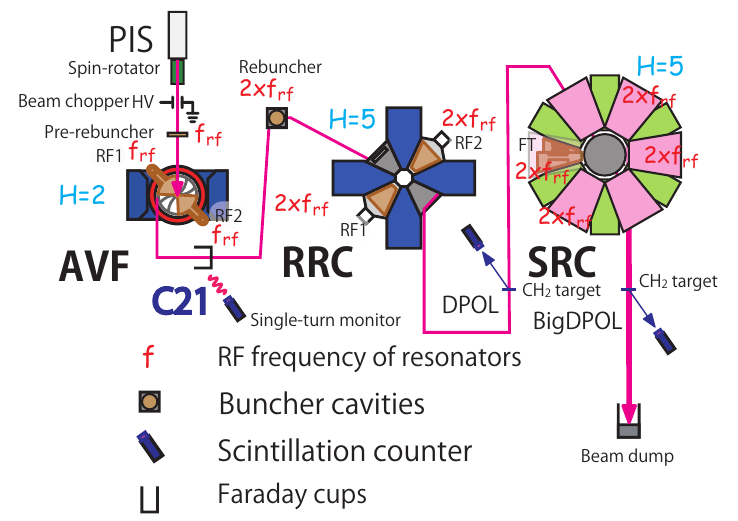
\includegraphics[width=0.74\textwidth,height=48mm,keepaspectratio]{../../physics/polarization_production_transport/figures/sakamoto2016_p1_fig1.png}\par
{\color{Muted}\fontsize{11}{14}\selectfont Historical accelerator layout showing DPOL before SRC and BigDPOL after SRC}
\end{center}
\vspace{1mm}
\smalltext
\begin{tabularx}{\textwidth}{@{}p{38mm}p{71mm}Y@{}}
\toprule
Location & What it measures & Questions for use\\
\midrule
After AVF & Source modes & Calibration at AVF energy. Dedicated measurement or inline monitoring?\\
After RRC & Before SRC & DPOL access. Calibration and target effects on SRC injection.\\
After SRC & Final beam energy & Space, count rate, and permitted attenuation before F3.\\
\bottomrule
\end{tabularx}\par
\vspace{3mm}
\textbf{First enquiry: existing DPOL after RRC.}\quad After-SRC installation remains an option.
\source{Sources: \src{\sakamoto}{Sakamoto et al., 2016, Fig. 1}; \src{\avftest}{Sugahara et al., INPC 2025, AVF polarimeter and Faraday-cup test}. Relating any upstream measurement to the SAMURAI target requires a transport check.}
\note{\notefour}
\end{frame}

\begin{frame}[t]{Beam attenuation before F3}
\lead{F3 total beam rate: $\dot N_{\mathrm{F3}}\leq10^7$ particles/s}
{\smalltext Proposed order, subject to beamline and interlock approval:\par}
\vspace{0mm}
\[
\mathrm{SRC}\ \longrightarrow\ \mathrm{polarimeter}\ \longrightarrow\ \mathrm{attenuation}\ \longrightarrow\ \mathrm{F3}\ \longrightarrow\ \mathrm{SAMURAI}
\]
\vspace{1mm}
\begin{columns}[T,onlytextwidth]
\column{0.48\textwidth}
\textbf{ATT: mesh beam attenuator}\par
\vspace{2mm}
\smalltext
Open apertures transmit part of the beam.\par
\vspace{2mm}
Nominal ratios: $1/2$, $1/3$, $1/5$, $1/10$, $1/100$.\par
\vspace{2mm}
Documented locations: C22, S31a and S64, upstream of RRC.\par
\vspace{2mm}
Upstream attenuation also lowers the after-SRC count rate.
\column{0.48\textwidth}
\textbf{Slits: acceptance restriction}\par
\vspace{2mm}
\smalltext
Select position, angle, or momentum.\par
\vspace{2mm}
F2--F3 angular-selection slits are documented.\par
\vspace{2mm}
Reduction depends on the beam distribution and aperture settings.\par
\vspace{2mm}
Assess stability, intercepted beam, and the polarization of the transmitted fraction.
\end{columns}
\vspace{2mm}
{\smalltext\color{Rust}\textbf{Interlock condition:} the 2025 BIS report describes an upstream-ATT check for primary-beam delivery. Downstream slits alone cannot be assumed to satisfy it.}
\source{Sources: \src{\fthreelimit}{BigRIPS F3 instructions}; \src{\attguide}{RIKEN intensity guide, p. 7}; \src{\attlocations}{APR 47 (2014), p. 156}; \src{\slitsource}{APR 52 (2019), p. 130}; \src{\bis}{APR 58 (2025), pp. 98--99}. Confirm the applicable operating mode and current interlock configuration.}
\note{\notefive}
\end{frame}

\begin{frame}[t]{Decisions for beam preparation}
\smalltext
\renewcommand{\arraystretch}{1.2}
\begin{tabularx}{\textwidth}{@{}p{48mm}Y@{}}
\toprule
Topic & Agreement needed from the meeting\\
\midrule
RIKEN capability & Independent tuning without Prof. Sekiguchi's help. Responsible RIKEN team and preparation time.\\[2mm]
Polarization mode & Pure tensor RF recipe, residual $p_y$ tolerance, and vertical transport without additional Wien rotation.\\[2mm]
Polarimeter & Existing AVF/RRC device or after-SRC installation. Monitoring interval and target-side cross-check.\\[2mm]
Beam intensity & Attenuation location, ATT/slit settings, and applicable F3 interlock conditions.\\
\bottomrule
\end{tabularx}\par
\vspace{6mm}
\lead{Count-rate requirement to quantify}
\vspace{-2mm}
\(R_{\rm useful}=\dot N_{\rm pol}\,n_t\,\sigma_{\rm acc}\,\epsilon\,f_{\rm live}\)\par
\vspace{3mm}
\smalltext
Agree on beam energy, intensity, target thickness, and the required $p_{yy}$ uncertainty within a specified time.\par
\vspace{2mm}
\textbf{Higher useful counts shorten the monitoring interval.} Analyzing power and backgrounds also determine the precision.
\source{Discussion requests for this experiment. Rate expression assumes a thin target and effective acceptance/efficiency factors. No beam-delivery or precision value is assumed.}
\note{\notesix}
\end{frame}
\fi
\end{document}
